\documentclass[11pt,border=5pt]{standalone}
\usepackage{fontspec}
\setmainfont{cmunrm.otf}[BoldFont=cmunbx.otf,ItalicFont=cmunti.otf,BoldItalicFont=cmunbi.otf]
\usepackage{amsmath}
\usepackage{unicode-math}
\setmathfont{NewCMMath-Regular.otf}
\usepackage{tikz}
\usetikzlibrary{arrows.meta,patterns,angles,quotes}
\begin{document}
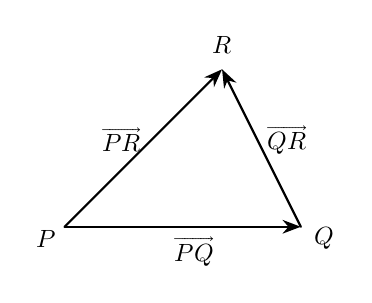
\begin{tikzpicture}[>=Stealth,font=\small,line cap=round,line join=round]
\coordinate (P) at (0,0);\coordinate (Q) at (3,0);\coordinate (R) at (2,2);
\draw[->,thick] (0,0) -- (3,0) node[pos=0.55,below] {$\overrightarrow{PQ}$};
\draw[->,thick] (3,0) -- (2,2) node[pos=0.55,right] {$\overrightarrow{QR}$};
\draw[->,thick] (0,0) -- (2,2) node[pos=0.55,left] {$\overrightarrow{PR}$};
\node at (-0.25,-0.15) {$P$};
\node at (3.3,-0.15) {$Q$};
\node at (2,2.3) {$R$};

\end{tikzpicture}
\end{document}
